\section{Lezione 28 - 24/11/2023}
\subsection{Max/Min Heap}
Max/Min Heap è un albero binario \textbf{completo} (ogni foglia di trova a profondità $h$ o $h-1$, ogni nodo interno tranne al massimo uno ha grado 2) in cui ogni nodo ha valore maggiore/minore uguale al valore dei sui figli.
\begin{figure}[H]
	\centering
	\begin{subfigure}[b]{0.60\textwidth}
		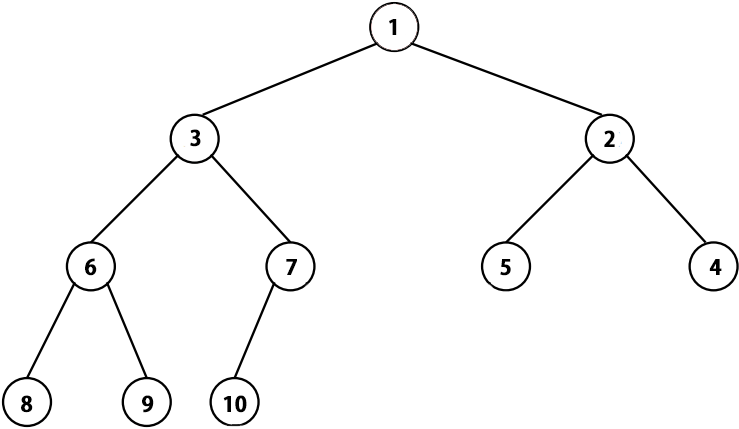
\includegraphics[width=\textwidth]{MinHeapv.png} 
		\caption*{MinHeap}
	\end{subfigure}
\end{figure} 
\paragraph{Proprietà} Nel Max/Min Heap il max/min è in radice (tempo costante) 



%Come per i BST nel caso di elimazione di un nodo (esempio la radice) bisogna andare a "ricostruire" lo heap, 

\subsubsection{Altezza di uno Heap (Albero Completo)}
Prendiamo un albero completo di altezza $h$:
\begin{figure}[H]
	\centering
	\begin{subfigure}[b]{0.40\textwidth}
		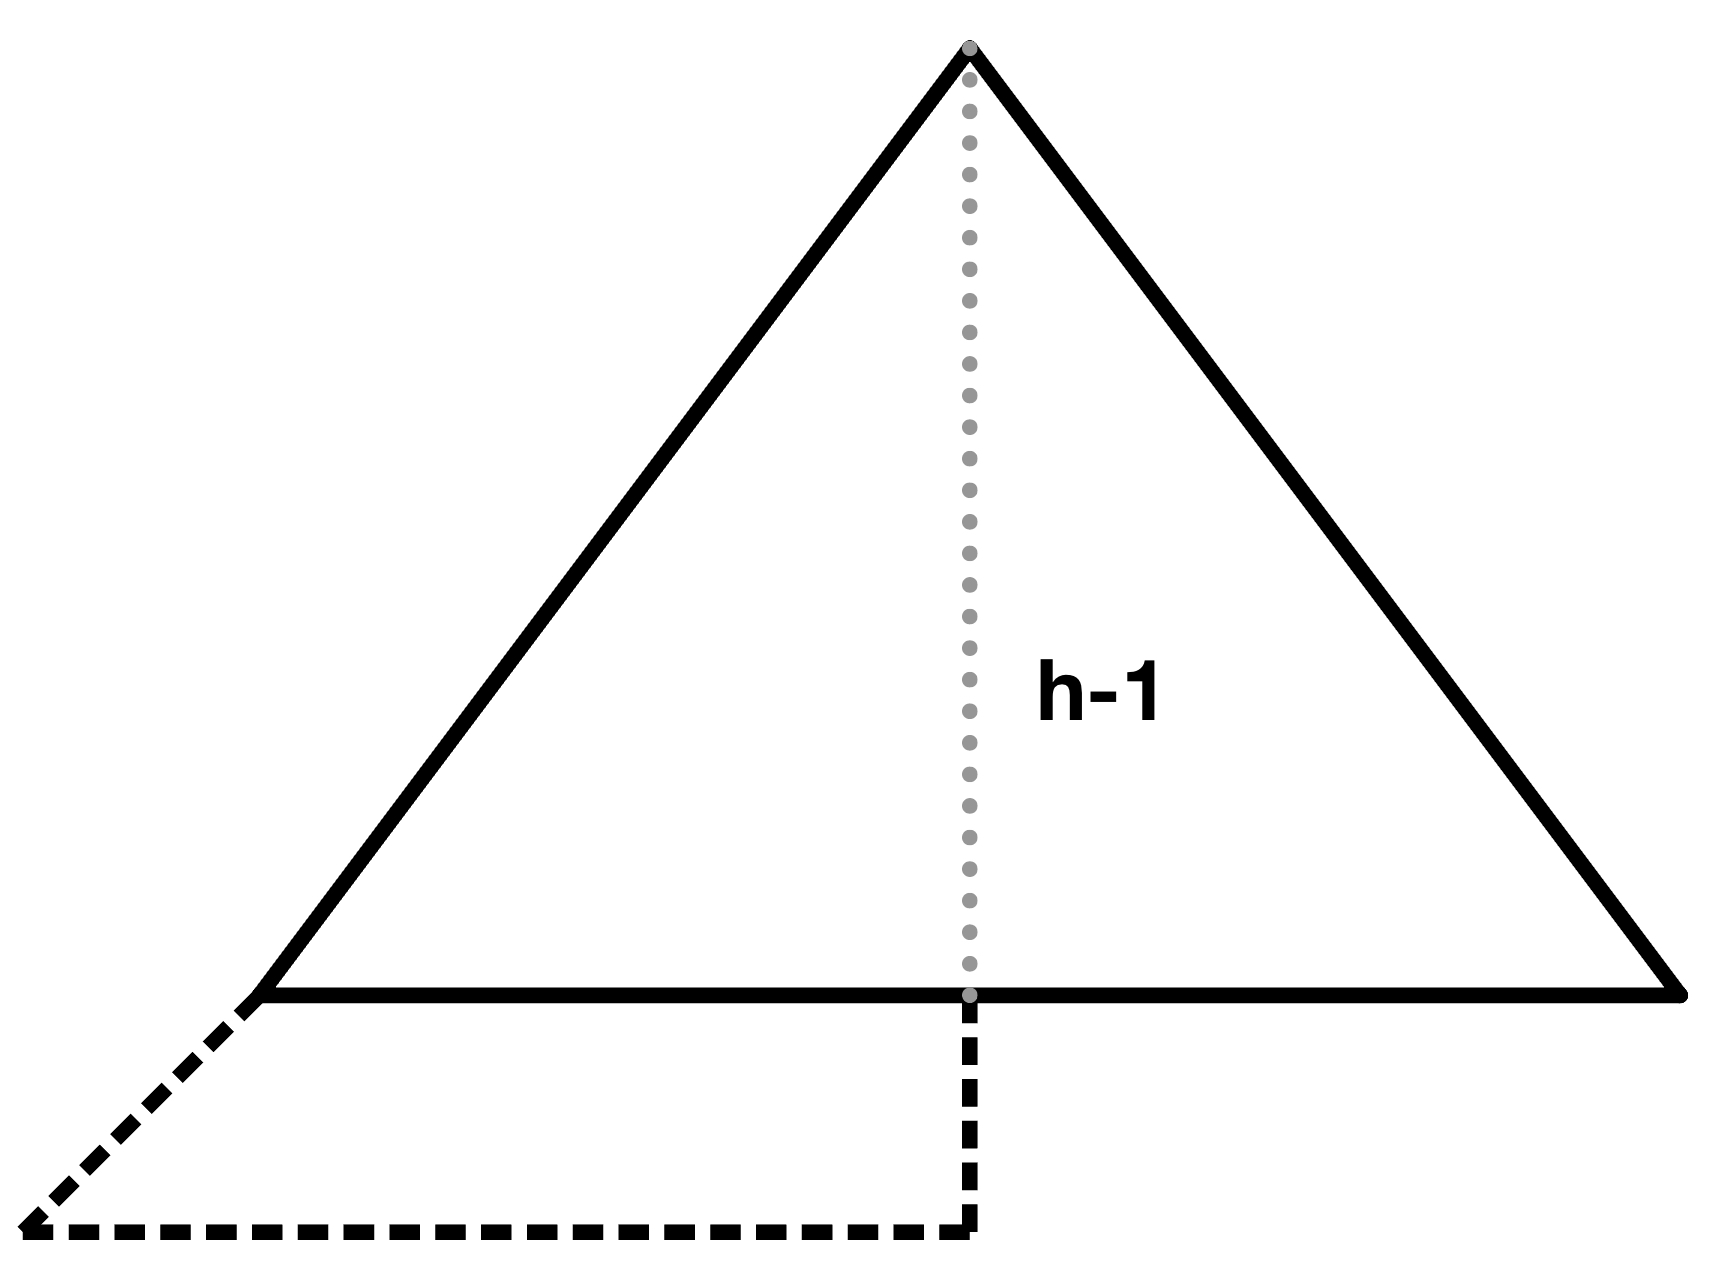
\includegraphics[width=\textwidth]{AlberoCompleto.PNG} 
	\end{subfigure}
\end{figure} 
Il "sottoalbero" $h-1$ è un albero pieno quindi contiene $2^h-1$ nodi.\smallskip

L'ultimo livello cioè $h$ sappiamo che contiena almeno un nodo quindi i nodi di un albero pieno $+1$ cioé $(2^h-1 +1)$, quindi avremo:
$$ \underbrace{2^h}_{\text{min. nodi albero compl.}} \le n \le \underbrace{2^{h+1}-1}_{\text{max. nodi albero compl.}}$$
Possiamo riscriverlo nel seguente modo:
$$ 2^h \le n < 2^{h+1} $$
Andiamo ad applicare il logaritmo:
$$ \log_2(2^h) \le \log_2 n < \log_2(2^{h+1})$$
Andando a svolgere i logaritmi abbiamo:
$$ h \le log_2 n < h+1$$
Da qui segue (arrotondando per difetto) che:
$$ h=[log_2 n]$$

\subsection{Rappresentare un albero tramite Array}
Un altro modo per poter rappresentare un albero è tramite l'ausilio di un array, in cui ogni cella corrisponderà ad un nodo con un indice $i$ e tramite quest'ultimo possiamo risalire ai suoi figli o genitore:\medskip

\begin{itemize}
    \item FiglioSX(i)=$2i$\smallskip
 
    \item FiglioDX(i)=$2i+1$\smallskip

    \item Parent(i)=$\frac{i}{2}$\smallskip

\end{itemize}
GLI INDICi PARTONO DA 1 NON DA 0 NON HO VOGLIO DI RIFARE L'IMMAGINE
\begin{figure}[H]
	\centering
	\begin{subfigure}[b]{0.40\textwidth}
		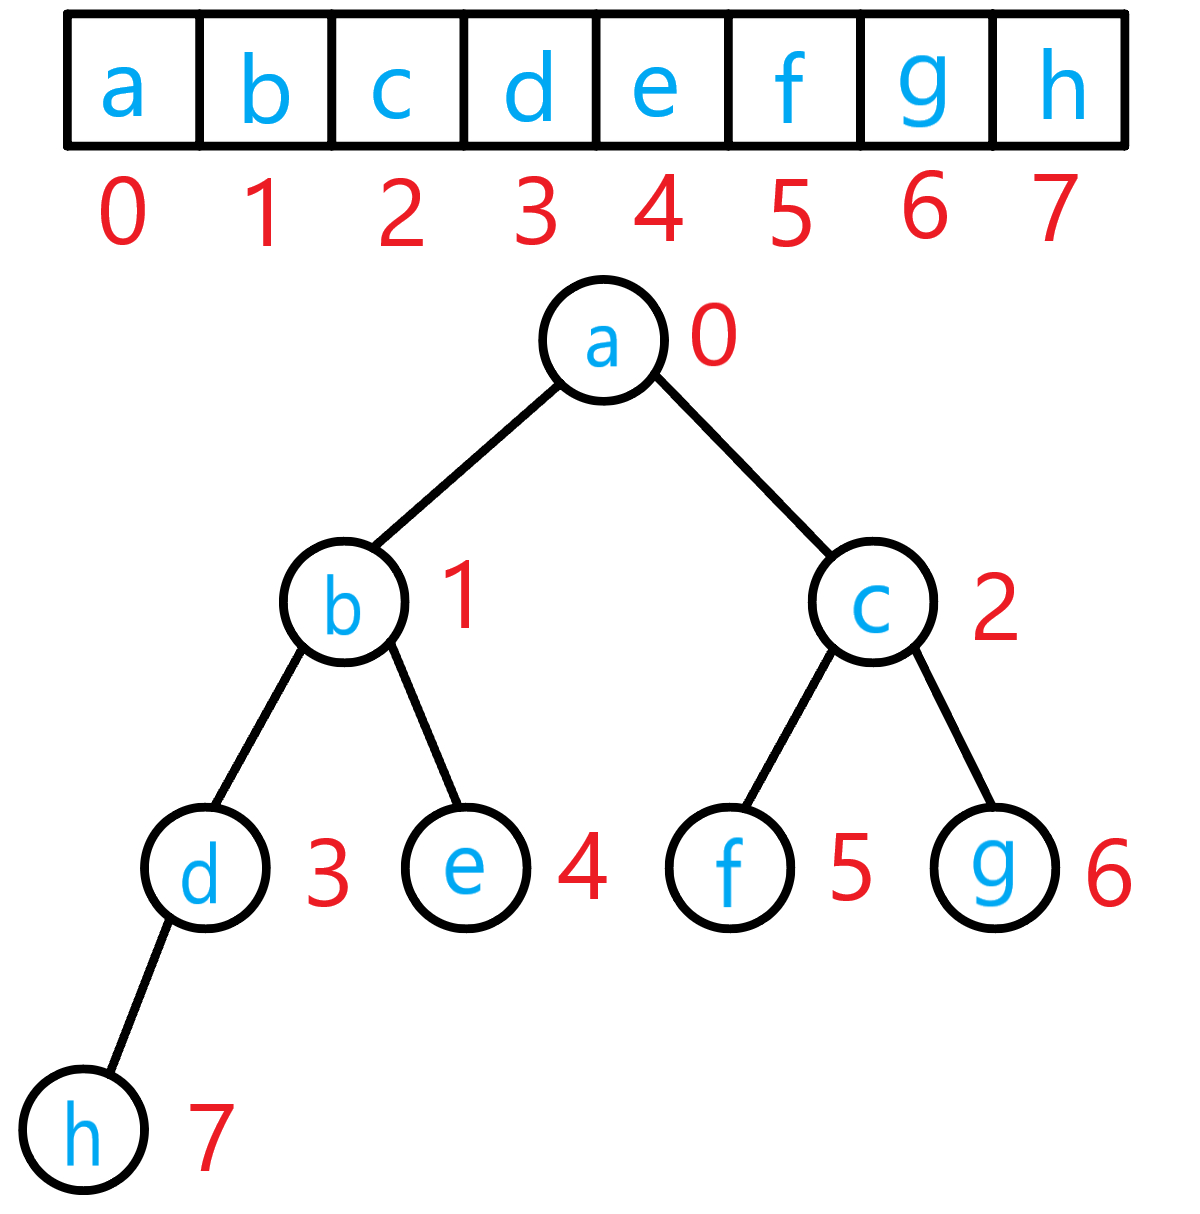
\includegraphics[width=\textwidth]{ArrayToTree.png} 
		%\caption*{MinHeap}
	\end{subfigure}
\end{figure} 
Per la nostra rappresentazione di Max/Min Heap andremo ad usare proprio un array.

\subsection{Rimozione Heap}
Rimuovere un nodo da uno Heap non è neccasseriamente un problema, esempio la rimozione di una foglia è abbastanza sicura (anche se possono violare delle proprietà), diverso se vogliamo rimuovere il max/min poiché andiamo a togliere la radice, quindi necessitiamo di una funzione per ripristinare lo heap.

\subsubsection{Heapify}
La funziona Heapify ripristina la proprietà di Heap al sottoalbero radicato nella posizione i, assumendo che i suoi sottoalberi destro e sinistro siano già degli Heap.
\begin{lstlisting}[language=Java]
Heapify(Q,i): //Q: albero come array, i: posizione sottoalbero
    j=sx(i) //indice figlio sinistro
    k=dx(i) //indice figlio destro 
    //Se il figlio sinistro e' piu' piccolo del padre e' min
    if j <= Q.size AND Q[j].val < Q[i].val then
        min=j 
    else //altrimenti il min e' il padre
        min=i 
    //se il figlio destro e' piu' piccolo del min' precedente 
    if k <= Q.size AND Q[k].val < Q[min].val then
        min=k //allora lui diventa il min
    //se il min non e' il padre
    if min != i then 
        SCAMBIA Q[i] CON Q[min] //scambiamo min(sx o dx) col padre
        Heapify(Q, min) //chiamata ricorsiva sull'indice min (sx o dx)
\end{lstlisting}
Ricorsivamente questo algoritmo andrà a ripristinare l'intero heap, il costo di sarà $log_2 n$.

\subsubsection{ExtractMin}
Andiamo a vedere proprio il caso di cui parlavamo cioè di estrattare il valori in radice (in questo caso il min) e andare ad "aggiustare" l'heap:
\begin{lstlisting}[language=Java]
Extract_Min(Q): //Q: albero come array
    if Q.size >0 then
        ret=Q[1] //la radice (min)
        Q[1]=Q[Q.size] //mettiamo come radice l'ultima foglia
        Q.size=Q.size-1 
        Heapify(Q,1) //Heapify su radice (1) per aggiustire l'heap 
    else 
        ret=NIL 
    return ret
\end{lstlisting}
Tutte queste operazione sono costanti ma dobbiamo aggiungere il costo di Heapify.

\subsection{Inserimento Heap}
Per andare ad inserire i valori nello heap andiamo a considerare ogni valore come una coppia formato da (valore, priorità), 
\begin{lstlisting}[language=Java]
DecreaseKey(Q,i,k): //Q: array, i: indice attuale, k: valore
    if Q[i].val > k then 
        O=Q[i].obj //oggetto coppia
        while i > 1 AND Q[Parent(i)].val > k DO 
            Q[i]=Q[Parent(i)]
            i=Parent(i)
        Q[i]=(O,k)
\end{lstlisting}